\chapter[The Effects of Increased NSB on the FD Trigger and Reconstruction]{\centering The Effects of \\ Increased Night Sky Background on \\ the Fluorescence Detector's Trigger and Reconstruction \\ }\label{Ch:SelectEff}

\section{Motivation}

The Pierre Auger Observatory has been operational since 2004 and the Collaboration is in the process of rolling out upgrades to improve the experiment. The current upgrade has been name AugerPrime \textbf{(ref)} and is a large project to improve both the Surface Detectors (SD) and the Fluorescence Detectors (FD). The FD portion of AugerPrime involves extending the duty cycle to observe Extensive Air Shower (EAS) events while the moon is above the horizon. The main purpose for extending the FD duty cycle to include observation times while the moon is visible is to increase the statistics per year for EAS events at the highest energy ($>$ 10$^{19.5}$ eV). 

In this chapter I use real data events and simulations to explore the effects of increasing the Night Sky Background (NSB) on the collaboration's reconstruction method and trigger efficiency. A real data set was used to evaluate the efficiency of the reconstruction method under different NSB intensities by artificially adding extra noise to signal traces. This method follows a study done by M. Unger \textbf{Find ref.}. The method from M. Unger study was used as a basis. The results where examined in depth and found to mainly test the robustness of the collaboration's reconstruction algorithm. This analysis led to the use of the collaboration FD simulations to evaluate the effects of the increased NSB on both the FD triggers and reconstruction efficiency.

\section{Background Information}

\subsection{Current Fluorescence Detector Operation}

Currently an Fluorescence Detector (FDs) run is organised for nights when the illuminated fraction of the moon is less than 70\% and the night has a minimum of 3 hours of operation with the moon below the horizon. The FD telescope shutters are opened when the sun is below -18\textdegree \ of the horizon (beginning of astronomical twilight). The FD shutters remain open while the average variance across the FD camera is less than 100 ADC$^2$/100 ns and the variance of no individual pixels (which are photomultiplier tubes) is greater than 2000 ADC$^2$/100 ns. ADC units is the digitised of the photomultiplier tube (PMT) anode signal in electrons to Analogue-to-Digital Converter (ADC) units and 100 ns is chosen as the time interval that the ADC is digitised over. The FD shutters at each site automatically close if the individual rain sensors are triggered or the measured wind speed is above 50 km/h at the individual FD sites. Using these guidelines the expected yearly FD duty cycle can be calculated. This calculation was performed by the collaboration in \textbf{DATE \& ref} to estimate the theoretical the FD duty cycle and the result is shown in Table \ref{tab:FD_uptime}. Bad weather is mainly caused by rain, high wind speeds or lightning strikes in the FDs field of view. Failures include any software or hardware issues that prevented any of the FD telescopes from collecting data.

\begin{table}[h]
\centering
\begin{tabular}{ c c }
\hline\hline
Theoretical up time & 22\% \\
Loss due to short nights ($<$ 3 hrs) & -2\% \\
Loss due to bad weather or failures & -5\% \\ \hline \hline
Total measurement time & 15\% \\
\hline\hline
\end{tabular}
\caption{Calculation of the yearly expected FD duty cycle done by the Collaboration. Bad weather is the inclusion of rain, high wind speeds and lightning strikes in the FDs field of view. Failures include any software or hardware issues that prevented any of the FD telescopes from collecting data.} \label{tab:FD_uptime}
\end{table}


Photons that enter the FD telescope pass through the optics, are converted to photo-electrons by PMT and are then converted to Analogue-to-Digital Converter units by the electronics. A basic diagram of how photons detected by an FD telescope are converted to ADC is shown in Fig. \ref{fig:FD_CoefficientLayout_PhotonToADC}. The steps are split into 3 parts: the optics, PMT and electronics. When the photon reaches the PMT it produces a photo-electron and the electron signal from the PMT is converted to ADC units by the electronics. 

\begin{figure}
\centering
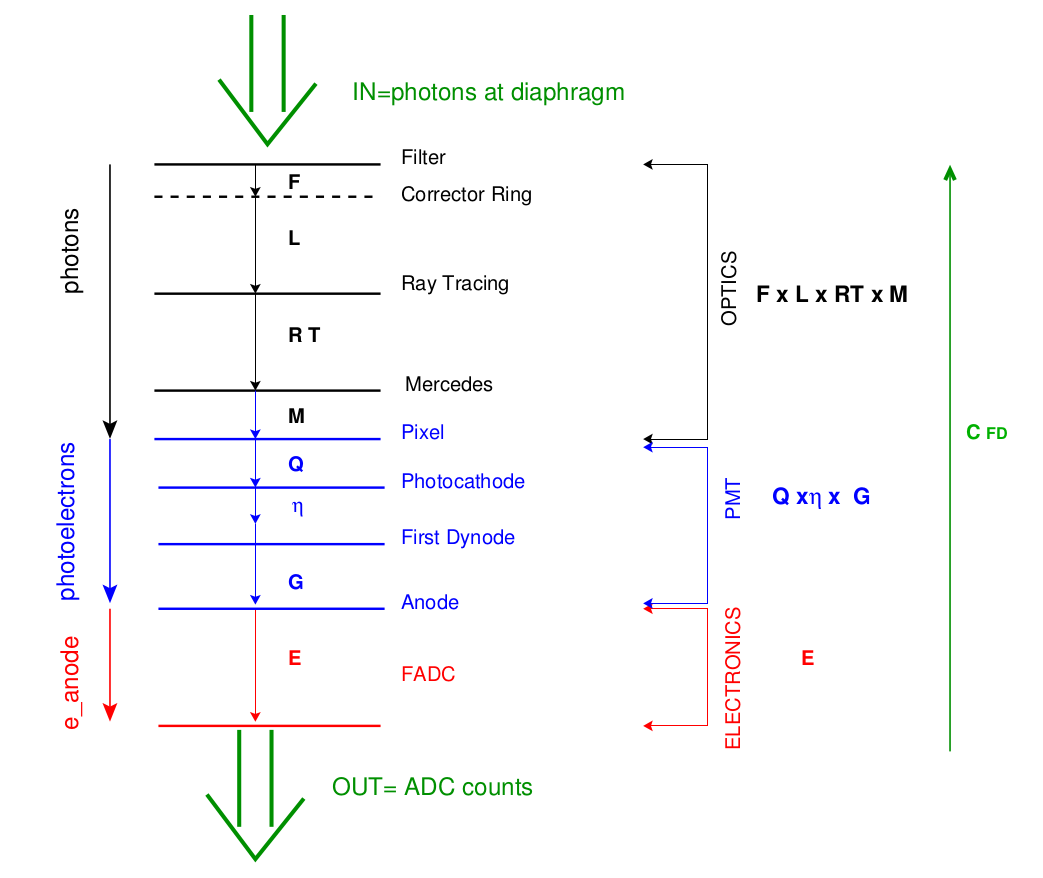
\includegraphics[width=\textwidth]{/home/tsudholz/PhD/Thesis/chapters/pix/SelEff/Layout_Coefficients_PhotonsToADC.png}
\caption{A diagram showing the steps that a photon passing through an FD telescope diaphram will travel to be convert to an ADC. The steps are split into 3 parts: the optics, PMT and electronics. When the photon reaches the PMT it is converted to a photo-electron and the electron signal from the PMT anode is converted to ADC units by the electronics.
- Define all of the symbols.} \label{fig:FD_CoefficientLayout_PhotonToADC}
\end{figure}
  
The electron signal from the FD PMT is AC coupled, which means the average ADC of the NSB is zero. Instead the ADC variance is used to measure the number of photons at the diaphragm. When converting a NSB trace into a NSB photon count the NSB ADC variance is proportional to the variance in the NSB photon count. To find the ADC variance due to the NSB the electronic noise has to be removed from the background ADC variance traces. Removal of the electronic noise is achieved by using Eq. \ref{eq:back_vars}. 
\begin{equation}
\left[\sigma^2_{\mathrm{ADC}}\right]^{\mathrm{sky}} = \left[\sigma^2_{\mathrm{ADC}}\right]^{\mathrm{back}} - \left[\sigma^2_{\mathrm{ADC}}\right]^{\mathrm{elec}} \label{eq:back_vars}
\end{equation} 
where:
\begin{itemize}
\item[] $\left[\sigma^2_{\mathrm{ADC}}\right]^{\mathrm{sky}}$ is the variance (ADC$^2$/100 ns) caused by the NSB.
\item[] $\left[\sigma^2_{\mathrm{ADC}}\right]^{\mathrm{back}}$ is the variance (ADC$^2$/100 ns) of background signal which is the combination of NSB and electronic noise.
\item[] $\left[\sigma^2_{\mathrm{ADC}}\right]^{\mathrm{elec}}$ is the variance (ADC$^2$/100 ns) of the electronic noise. The variance of FD electronic noise is measured while the shutters are closed.
\end{itemize}
The typical mean ADC variance of the NSB measured by Auger \ref{find} at Malargue is:
\begin{equation}
\left[\sigma^2_{\mathrm{ADC}}\right]^{\mathrm{sky}} = 25 \ \mathrm{ADC}^2 \ / \ 100 \ \mathrm{ns} \nonumber
\end{equation}

The variance in ADC$^2$ seen by the FD can be converted back to photon numbers at the diaphragm by the FD pixel calibration constant C$_{\mathrm{FD}}$ (photons/ADC units). The FD pixel calibration constant has been determined by illuminating the diaphragm with a known number of photons. This was originally done by a drum calibration which used a large device that covered the entire FD diaphragm and could illuminate the whole camera with a known number of diffuse photons. The drum calibration has now been retired and has been replaced with an experiment called the XY scanner [ref]. The XY scanner illuminates one pixel at the time and scans over the entire camera. The advantages of the XY scanner is that it is a more compact experiment with the aim of having the ability to be deployed more often to find the absolute calibration.

The FD pixel calibration factor C$_{\mathrm{FD}}$ can be used to find the variance of the NSB photons at the diaphragm from the measured ADC variance. An average variance of the NSB measured by an FD telescope under standard operational guidelines is $\sigma^2_{\mathrm{ADC}}$ = 25 ADC$^2$ / 100 ns. The calculations to work out the variance of the photon count (RMS$_{\mathrm{ph}}$ / 100 ns) from the measured variance in ADC$^2$ is as follows:
\begin{equation}
\mathrm{\sigma}^2_{\mathrm{ph}} = (\mathrm{C}_{\mathrm{FD}})^2 \times \sigma^2_{\mathrm{ADC}} \label{eq:varADC_to_RMSphotons}
\end{equation}
Using Eq. \ref{eq:varADC_to_RMSphotons} and C$_{\mathrm{FD}}$ = 4.5 photons / ADC, the average fluctuations on the photon count can be calculated.
\begin{equation}
\sigma_{\mathrm{ph}} = 23 \ \mathrm{photons} \ / \ 100 \ \mathrm{ns} \nonumber
\end{equation}
where $\sigma_{\mathrm{ph}}$ is the fluctuations on the photon count per 100 ns.

Finding the number of photons at the diaphragm takes more steps since the fluctuations are affected by more then the Poisson statistics of the photon number. The first step involves converting the ADC variance to photo-electron numbers. This step is achieved through using the combination of Eq. \ref{eq:numberPE} and Eq. \ref{eq:simgaPE}.
\begin{eqnarray}
\mathrm{n}_{\mathrm{pe}} &=& \frac{\sigma^2_{pe}}{(1 + \mathrm{V}_{\mathrm{G}})} \label{eq:numberPE} \\
\sigma^2_{pe} &=& [\sigma^2_{\mathrm{ADC}}]^{\mathrm{sky}} \ / \ \mathrm{A}^2_{\mathrm{G}} \label{eq:simgaPE}
\end{eqnarray}
where $\sigma_{pe}$ is the standard deviation of the photo-electron count, n$_{\mathrm{pe}}$ is the photon-electron count, V$_{\mathrm{G}}$ is the PMT gain variance factor \ref{in GAP2004} and A$_{\mathrm{G}}$ is the absolute gain (ADC/photo-electron) of the PMT. A$_{\mathrm{G}}$ is equal to:
\begin{equation}\label{eq:abs_gain}
\mathrm{A}_{\mathrm{G}} = \eta \times G \times E 
\end{equation}
where
\begin{itemize}
\item[] $\eta$ is the PMT collection efficiency at the first dynode.
\item[] $G$ is the PMT gain.
\item[] $E$ is the electronic conversion constant (ADC per anode electron).
\end{itemize}
An equivalent quantity can be used to calculate $\mathrm{A}_{\mathrm{G}}$ and is:
\begin{equation}\label{eq:abs_gain_alt}
\mathrm{A}_{\mathrm{G}} = \frac{1}{\mathrm{C}_{\mathrm{FD}}\times \mathrm{f} \times \mathrm{Q}}
\end{equation}
where
\begin{itemize}
\item[] Q is the Quantum efficiency of the PMT turning photons into photo-electrons.
\item[] f is the photon collection efficiency of the telescope optics. The components that make up the telescope optics are shon in Table. \ref{tab:OpticsBreakdown}.
\end{itemize}

\vspace{3mm}
\begin{table}[h]
\begin{center}
\begin{tabular}{|c|c|}
\hline 
C$_{\mathrm{FD}}$ & 4.5 photons/ADC \\
\hline
Q & 0.29 \\
\hline
f & 0.494 \\
\hline
\end{tabular} 
\end{center}
\caption{Typical values for the constants used to calculate A$_{\mathrm{G}}$ which is the absolute gain (ADC/photo-electron). $\mathrm{C}_{\mathrm{FD}}$ is the FD pixel calibration constant, Q is the Quantum efficiency of the PMT turning photons into photo-electrons and f is the photon collection efficiency of the telescope optics.} \label{tab:CFD_Q_F}
\end{table} 

\begin{table}[h]
\centering
\begin{tabular}{|c|c|c|}
\hline
Photon Collection Efficiency & f & F $\times$ L $\times$ T $\times$ R $\times$ M \\ \hline
Filter Transmission & F & 0.83 \\ \hline
Corrector Ring lens Transmission & L & 0.90 \\ \hline
Mirror Reflectivity & R & 0.90 \\ \hline
Camera Shadow Factor & T & 0.79 \\ \hline
Mercedes Collection Efficiency & M & 0.93 \\ \hline
\end{tabular}
\caption{Breakdown of all the components that go into the FD photon collection efficiency. Photon Collection Efficiency = Filter Transmission $\times$ Corrector Ring lens Transmission $\times$ Mirror Reflectivity $\times$ Camera Shadow Factor $\times$ Mercedes Collection Efficiency ( f = F $\times$ L $\times$ T $\times$ R $\times$ M)}\label{tab:OpticsBreakdown}
\end{table}

Therefore A$_{\mathrm{G}}$ can be calculated from Eq. \ref{eq:abs_gain} using the values from Table \ref{tab:CFD_Q_F}. Typical measured values for C$_{\mathrm{FD}}$, Q and f shown in Table \ref{tab:CFD_Q_F}. The PMTs used as camera pixels in the FDs are HAMAMATSU XP3062 and are operated at a gain of $\sim$ 5 $\times$ 10$^4$ electrons/photo-electron.

The next step is to convert the photo-electron numbers to number of photons at the diaphragm. This step is achieved through using Eg. \ref{eq:numberPhotons}.
\begin{equation}
\mathrm{n}_{\mathrm{ph}} = \frac{\mathrm{n}_{\mathrm{pe}}}{\mathrm{Q} \times \mathrm{f}} \label{eq:numberPhotons}
\end{equation}

From all of the equations stated above the following table shows the expected photon count at the aperture per 100 ns from the measured variance (ADC$^2$ / 100 ns).
\begin{table}
\begin{center}
\begin{tabular}{| c | c | c | c | }
\hline \hline
\textbf{Moon Illumination} & \textbf{Variance} & \textbf{Photons / 100 ns} & \textbf{Photons / 100 ns} \\
\textbf{Fraction (\%)} &\textbf{(ADC$^2$/100 ns)} & \textbf{@ Pixel} & \textbf{@ diaphragm} \\
\hline \hline
0 & 25  & 23 & 46 \\
\hline
50 & 250  & 227 & 459 \\
\hline
100 & 2500  & 2267 & 4588 \\
\hline
\end{tabular}
\end{center}
\caption{}
\end{table}

\subsection{Night Sky Background and the Moon}

\begin{figure}
\centering
\begin{subfigure}[b]{0.60\textwidth}
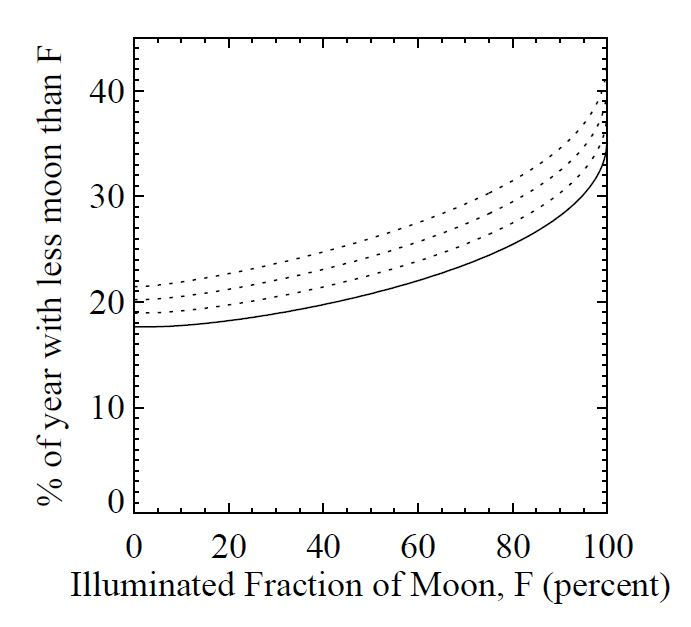
\includegraphics[width=\textwidth]{chapters/pix/SelEff/IlluminatedMoonFrac_Twilight.JPG}
\caption{}\label{fig:MoonYearlyFrac}
\end{subfigure}
\hspace*{3mm}
\begin{subfigure}[b]{0.90\textwidth}
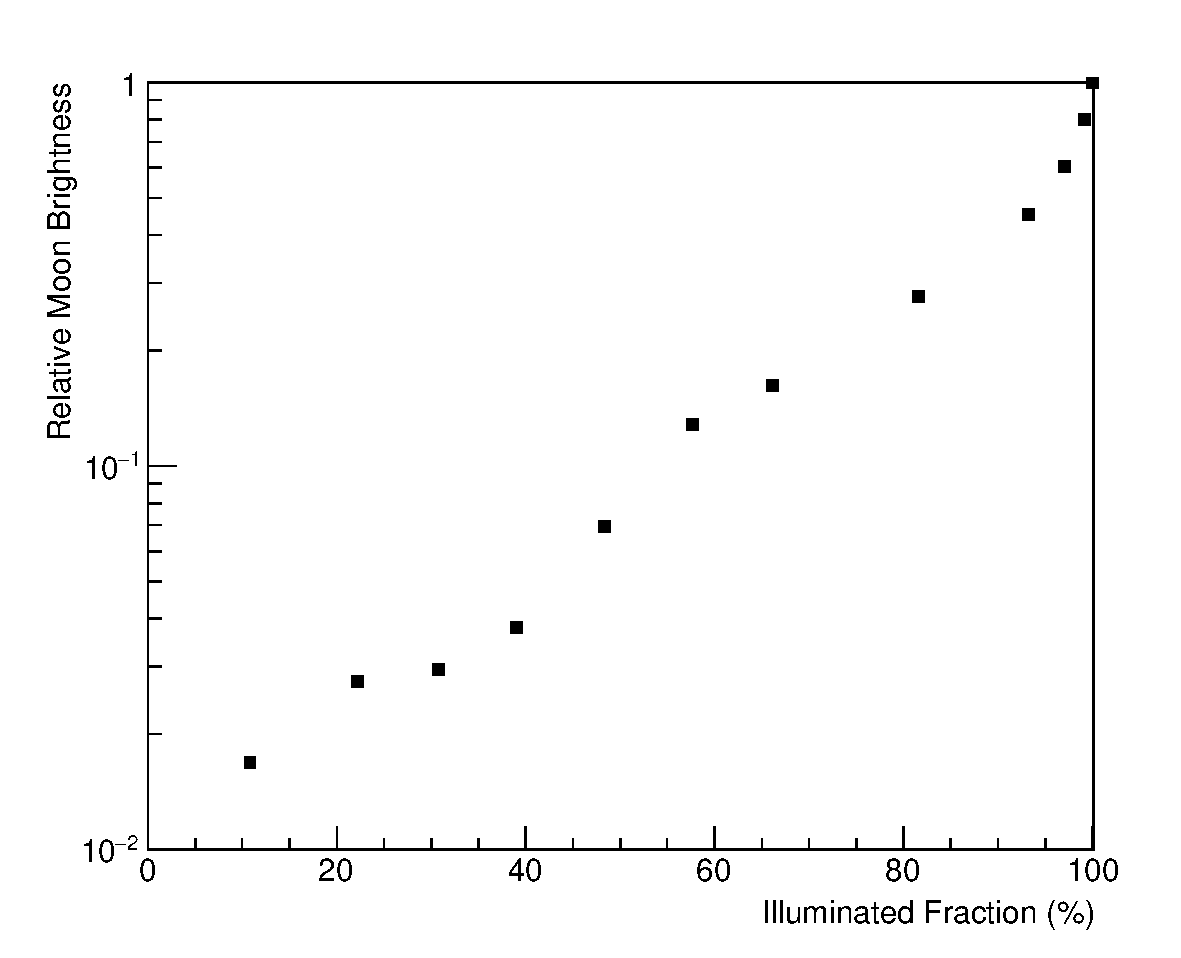
\includegraphics[width=\textwidth]{/home/tsudholz/PhD/Thesis/chapters/pix/SelEff/RelMoonBright_Vs_IllumFrac_LogScale.pdf}
\caption{}\label{fig:MoonIllumFrac}
\end{subfigure}
\caption{\textbf{(a)} Integral fraction of nights across the year with the moon with different illuminated fractions. Only times between dusk and dawn have been included. The solid line is the astronomical twilight (sun at least 18\textdegree \ below horizon). The dotted lines represent relaxed definitions of twilight with the sun being at 15\textdegree , 12\textdegree \ and 9\textdegree \ below the horizon. \textbf{(b)} Relative brightness of the moon in the night sky compared with a full moon as a function of illuminated fraction. Images taken from \textbf{ref{(GAP1996-034)}}. } 
\end{figure}

\begin{figure}
\centering
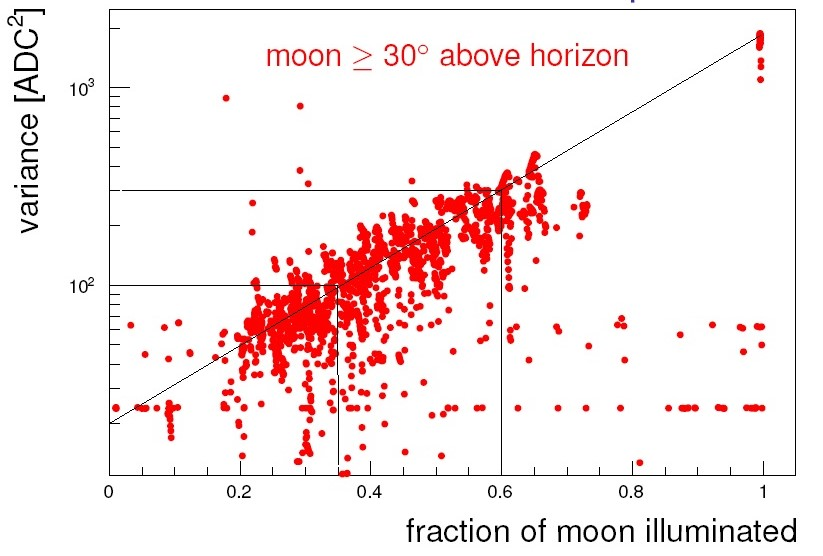
\includegraphics[width=0.80\textwidth]{chapters/pix/SelEff/BGLoop_Variance_crop.jpg}
\caption{Measured NSB variance from the Fluorescence Detectors at Standard PMT HV setting with different moon illuminated fractions. The moon was 30\textdegree \ above horizon or greater. Image taken from \textbf{ref(Radamir)}.} \label{fig:ADCvarVSmoonIllumFrac}
\end{figure}

The Night Sky Background for Auger typically refers to airglow, zodiacal light, scattered starlight and any man-made light. Moonlight is a separate source of background light as an FD shift is typically operated when the moon is below the horizon. Table \ref{tab:MoonLightADC} shows the expected change in average background light observed by the FD telescopes for no moon, 1st/3rd quarter moon and full moon / twilight. 1st/3rd quarter moon is either one quarter or three quarters through the moon orbital cycle and is when 50\% of the observable moon from earth is illuminated. From the table it can seen that going from no moon to quarter moon to full moon jumps by a factor of ten in the observed ADC variance at each step. The large change in moon brightness for the different phases is due to the fact that the light is subject to spectral reflection not diffusion reflection.

\begin{table}[h]
\centering
\begin{tabular}{c c c c}
\hline\hline
Condition & Illumination Fraction & $\sigma^2$ [ADC$^2$/100 ns] & I$_{\mathrm{a}}$ [$\mu$A] \\ \hline\hline
no moon & 0\% & 25 & 0.5 \\
quarter moon & 50\% & 250 & 5 \\
full moon/twilight & 100\% & 2500 & 50 \\ 
\hline\hline
\end{tabular}
\caption{Expected average observed variance in ADC$^2$, and the anode current in $\mu$A by the PMTs in the FD telescopes under different NSB conditions. No Moon is the typical conditions for operation of the FD shift.} \label{tab:MoonLightADC}
\end{table} 

Figure \ref{fig:MoonYearlyFrac} plots the integral fraction of the night time within a year with the moon less than a particular illuminated fraction. Only times between astronomical dusk and dawn has been included. The solid line shows the percent of the year is astronomical twilight (sun at least 18\textdegree below the horizon. The dotted lines represent relaxed definition of twilight with the sun being at 15\textdegree , 12\textdegree \ and 9\textdegree \ below the horizon. The line curves up slowly due to that throughout the moon orbital cycle at times it will above the horizon during daylight hours. After first quarter and before 3rd quarter the moon be visible for longer at night time. Observing under indirect moonlight could increase the duty cycle by 5\% to 10\% across a year.


Figure \ref{fig:MoonIllumFrac} shows the relative change in brightness of the moon depending of the observed illuminated fraction. The red line is a fitted exponential to U-Band data taken at the La Palma observatory. The graph shows the large different in moon brightness as the illuminated fraction increases which was also described in Table \ref{tab:MoonLightADC}. The slope is comparable to actual data taken from the background files measured by the FD telescopes. The measured ADC variance plotted against fraction of illuminated moon is shown in Figure \ref{fig:ADCvarVSmoonIllumFrac}.


\subsection{Toy Model of the effect of increased NSB on aperture}

A simple measure of how well a detector will operate is to calculate the signal-to-noise (S/N) ratio. The steps that I followed was outlined in \ref{P. Sokolsky}. The signal-to-noise ratio is denote by:
\begin{equation}
\mathrm{Signal \ to \ Noise} = \frac{\mathrm{S}}{\mathrm{N}} \label{eq:SNratio}
\end{equation}
where S is the signal and N is the noise amplitude. The first step is to calculate the noise (N) expected from a background signal ($B$). First the background photo-electron count rate ($B$) seen from the night sky is calculate via:
\begin{equation}
B \propto \epsilon A b \Delta \Omega \Delta t \nonumber
\end{equation}
where $\epsilon$ is the optical efficiency of the telescope, $A$ is the mirror area, $b$ is the background light flux and $\Delta\Omega$ is the solid angle of the sky viewed by a single PMT. $\epsilon$ is f $\times$ Q where F is the optics factor shown in Table. \ref{tab:OpticsBreakdown} and Q is the quantum efficiency of the photon sensitive device (i.e. photomultiplier tube). Next the fluctuations on the noise can be found which is the square root of the background signal:
\begin{equation}
N = \sqrt{B} \propto \sqrt{\epsilon A b \Delta \Omega \Delta t} \label{eq:DetectNoise}
\end{equation}

Next step is to calculate the signal (S) from an extensive air shower that a detector would observe.
\begin{equation}
S \propto \frac{\epsilon A n_{+} n_{\gamma} c \Delta t}{4 \pi \mathrm{R}^2} e^{-\mathrm{R}/\lambda_{\mathrm{R}}} \label{eq:DetectSignal}
\end{equation}
where $n_+$ is the number of charge particles in the shower viewed by the photon sensitive device, $n_{\gamma}$ is the photon yield per charged particle for atmospheric scintillation, $R$ is the distance to the shower segment, $c\Delta t$ is the length of the shower segment, and $\lambda_{\mathrm{R}}$ is the Rayleigh attenuation length of light in the atmosphere. Substituting Eq. \ref{eq:DetectNoise} and Eq. \ref{eq:DetectSignal} into Eq. \ref{eq:SNratio} and removing the proportionality gives:
\begin{equation}
\frac{S}{N} = n_+ n_{\gamma} c \frac{(1 + \mathrm{cos}\theta)}{4 \pi (\mathrm{R} \times \mathrm{sin}\theta)^2} \sqrt{\frac{\epsilon A \Delta t}{b \Delta\Omega}} e^{-\mathrm{R}/\lambda_{\mathrm{R}}} \label{eq:SN_complete}
\end{equation}
where $\theta$ is the viewing angle of the EAS.

From here I use values specific to the Fluorescence Detectors to calculate the S/N ratio expected. The majority of the values used are shown in Table \ref{tab:FDvalues}. The viewing angle is 90\textdegree \ as the shower is viewed at 15\textdegree \ with the center of the FD camera at 15\textdegree \ elevation. As the perpendicular segment of the shower is being observed therefore R = R$_P$ where R$_P$ is the closest distance that the shower axis is to the FD. The Rayleigh attenuation length ($\lambda_{\mathrm{R}}$) is calculated via:
\begin{equation}
\lambda_{\mathrm{R}} = 2974 \left(\frac{\lambda}{400 \ \mathrm{nm}} \right)^4 \mathrm{g}/\mathrm{cm}^2 \label{eq:RayleighAttenuationLength}
\end{equation}
where $\lambda$ is the chosen wavelength in nanometres. Currently R$_P$ is in units of length where the Rayleigh attenuation length calculated in Eq. \ref{eq:RayleighAttenuationLength} in units of mass per length squared. A diagram of how R$_P$ and the shower axis is related to the detector is shown in Fig. \ref{fig:ShowerPlaneAndAxis}. To find the distance R$_P$ in terms of grammage the term $\Delta$X$_P$ is defined. Substituting this term into Eq. \ref{eq:SN_complete} becomes:
\begin{equation}
\frac{S}{N} = n_+ n_{\gamma} c \frac{(1 + \mathrm{cos}\theta)}{4 \pi (\mathrm{R} \times \mathrm{sin}\theta)^2} \sqrt{\frac{\epsilon A \Delta t}{b \Delta\Omega}} e^{-\Delta \mathrm{X}_P / \lambda_R}
\end{equation}
The $\Delta$X$_P$ can be calculated from the distance $R_P$ via
\begin{eqnarray}
\Delta \mathrm{X}_P &=& \Delta X_{vertical} / \mathrm{cos}75^{\circ} \\
\Delta \mathrm{X}_{\mathrm{vertical}} &=& 860 - 860\mathrm{exp}(-\mathrm{h}/7500) \\
\mathrm{h} &=& \mathrm{R}_P \times \mathrm{sin}15^{\circ}
\end{eqnarray}
where h is the vertical distance of the shower segment in meters and $\Delta$X$_{\mathrm{vertical}}$ is the vertical path in g/cm$^2$, the shower axis is at 15\textdegree \ elevation and 75\textdegree \ is the zenith angle. To find the grammage along the path to R$_P$ the vertical distance h is substituted and then the path $\Delta$X$_P$ can be found. The relationship between $\Delta$X$_P$ and R$_P$ is shown in Fig. \ref{fig:XpVsRp} for a detector viewing the sky at 15\textdegree \ elevation. The relationship is curved due to the amount of atmospheric molecules dropping off rapidly as the observed event moves further away both horizontally and vertically.


\begin{table}
\centering
\begin{tabular}{|c|c|c|}
\hline
optical efficiency & $\epsilon$ & 0.135 \\ \hline
mirror area & $A$ & 3.8 m$^2$ \\ \hline
Standard background light flux & $b1$ & 5e5 photons / m$^2$ / sr / $\mu$s \\ \hline
Increased background light flux & $b2$ & 5e6 photons / m$^2$ / sr / $\mu$s \\ \hline
solid angle of a single PMT & $\Delta\Omega$ & 5.38e-4 sr \\ \hline
viewing angle & $\theta$ & 90$^\circ$ \\ \hline
speed of light & $c$ & 3e2 m / $\mu$s \\ \hline
number of charged particles & $n_+$ & Particle Energy / 1e9 \\ \hline
Fluorescence yield & $n_{\gamma}$ & 4 photons / m / charged particle\\ \hline
Chosen wavelength & $\lambda$ & 350 nm \\ \hline
Rayleigh attenuation length & $\lambda_{\mathrm{R}}$ & 1743 g / cm$^2$ \\ \hline
\end{tabular}
\caption{Values specific to the Fluorescence Detectors.} \label{tab:FDvalues}
\end{table}

\begin{figure}
\centering
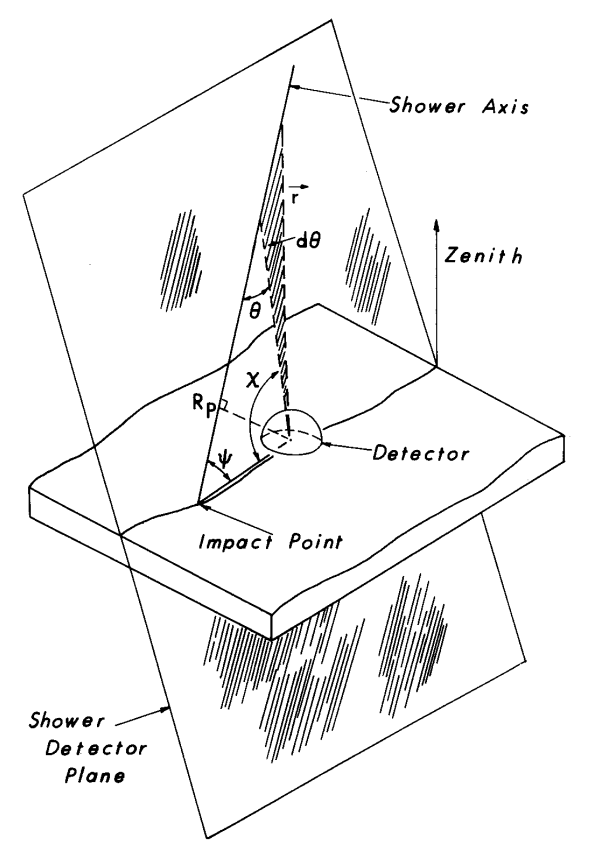
\includegraphics[height=0.45\textheight]{chapters/pix/SelEff/ShowerPlane_and_Detector.png}
\caption{Diagram showing the parameters used. Also show how they relate to the plane of the shower axis and to the position of the detector.} \label{fig:ShowerPlaneAndAxis}
\vspace{3mm}
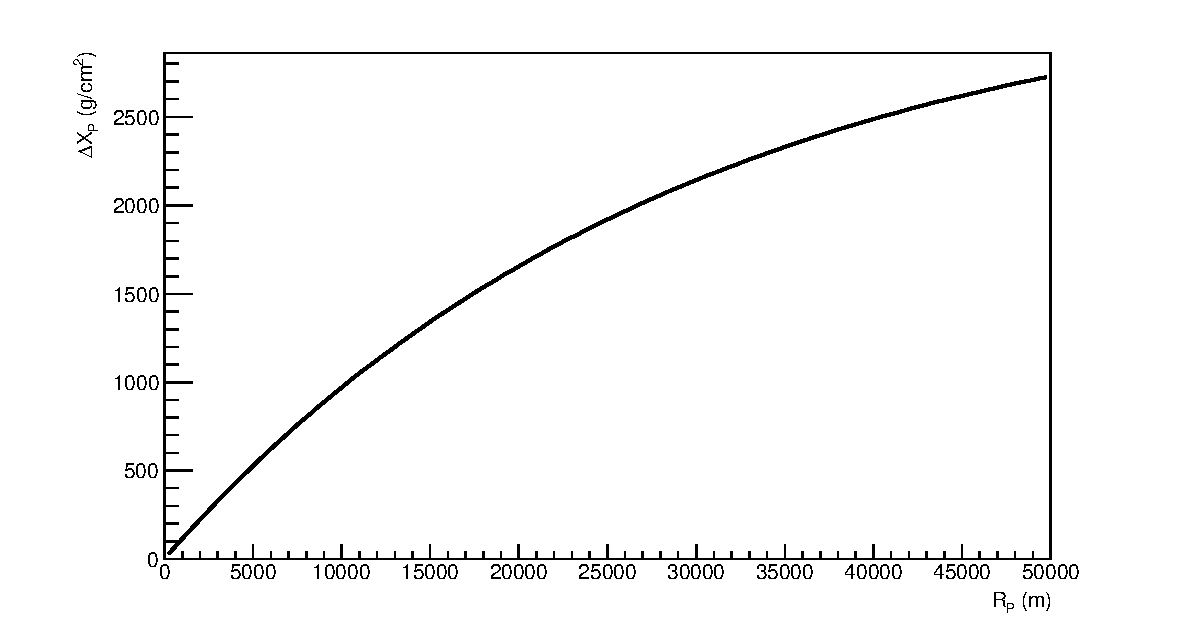
\includegraphics[width=\textwidth]{chapters/graphs/SelectionEff/XpVsRp.pdf}
\caption{How the relationship between the distance to the shower axis and grammage along the path. In this case the distance to the shower axis is denoted R$_P$ and the grammage is denoted $\Delta$X$_P$. R$_P$ is the closest distance that the shower axis is to the detector. The angle of the shower is 15$^{\circ}$} \label{fig:XpVsRp}
\end{figure}


\begin{figure}
\centering
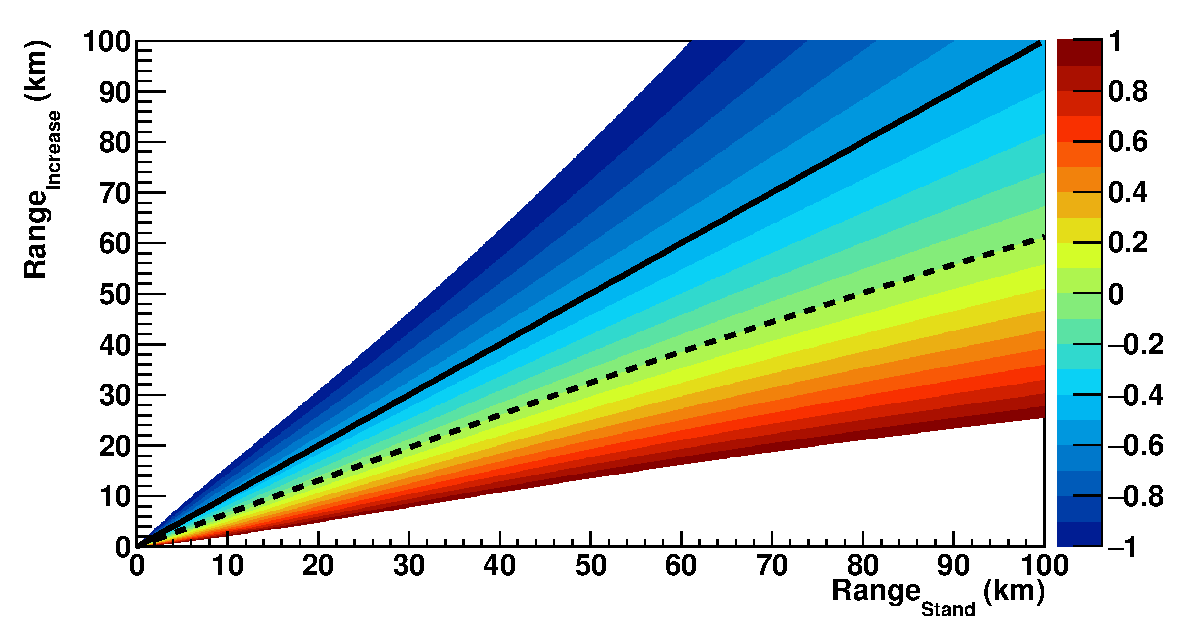
\includegraphics[width=\textwidth]{chapters/graphs/SelectionEff/RangeIncreaseVsRangeStand_Xp.pdf}
\caption{The image of the calculated Signal-to-Noise ratio the NSB at the Standard value and Increased NSB by a factor of 10 as a function of distance for an individual detector. The dashed black line denotes the distances where the Signal-to-Noise ratio is the same for the different NSB levles. The solid black line denotes where the distances are equal.}\label{fig:RangeIncVsRangeStand}
\includegraphics[width=\textwidth]{chapters/graphs/SelectionEff/RatioAreaVsDistance_Xp.pdf}
\caption{The image shows how the ratio of the detector viewing area changes with increasing the NSB by a factor of 10 as a function of distance from the detector. The solid black line denotes where the Signal-to-Noise ratio is the same.}\label{fig:RatioAreaVsDistance}
\end{figure}

\begin{figure}
\centering
\begin{subfigure}[b]{0.48\textwidth}
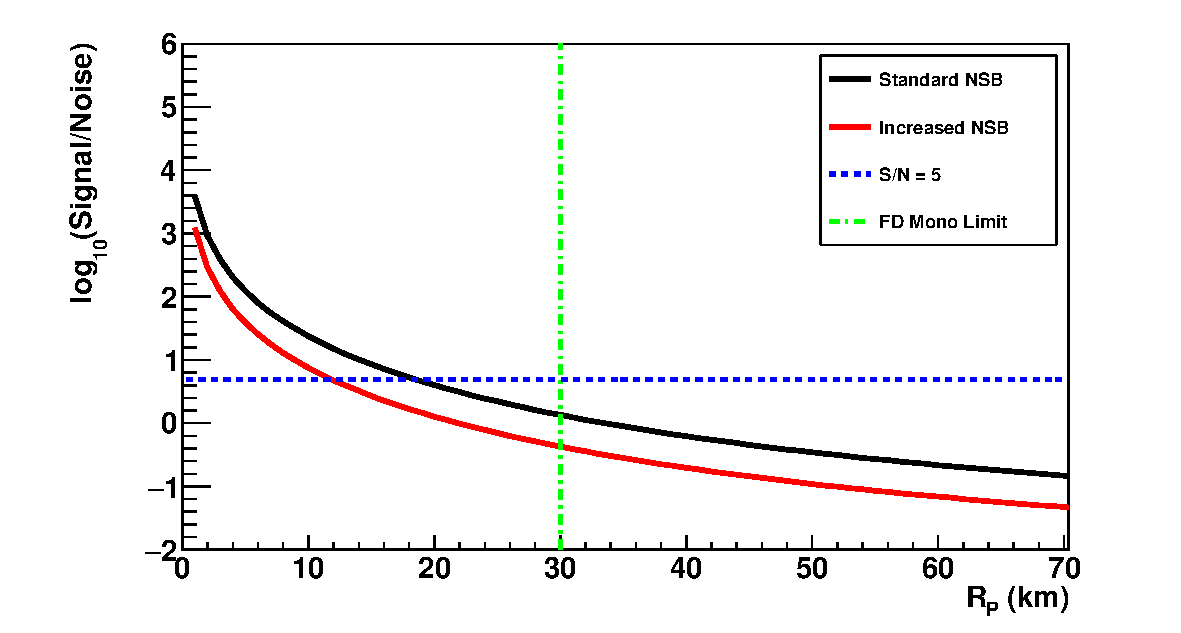
\includegraphics[width=\textwidth]{chapters/graphs/SelectionEff/SignalToNoiseVsDistance_E1e18eV.pdf}
\caption{E = 1 $\times$ 10$^{18}$ eV}
\end{subfigure}
\hspace{3mm}
\begin{subfigure}[b]{0.48\textwidth}
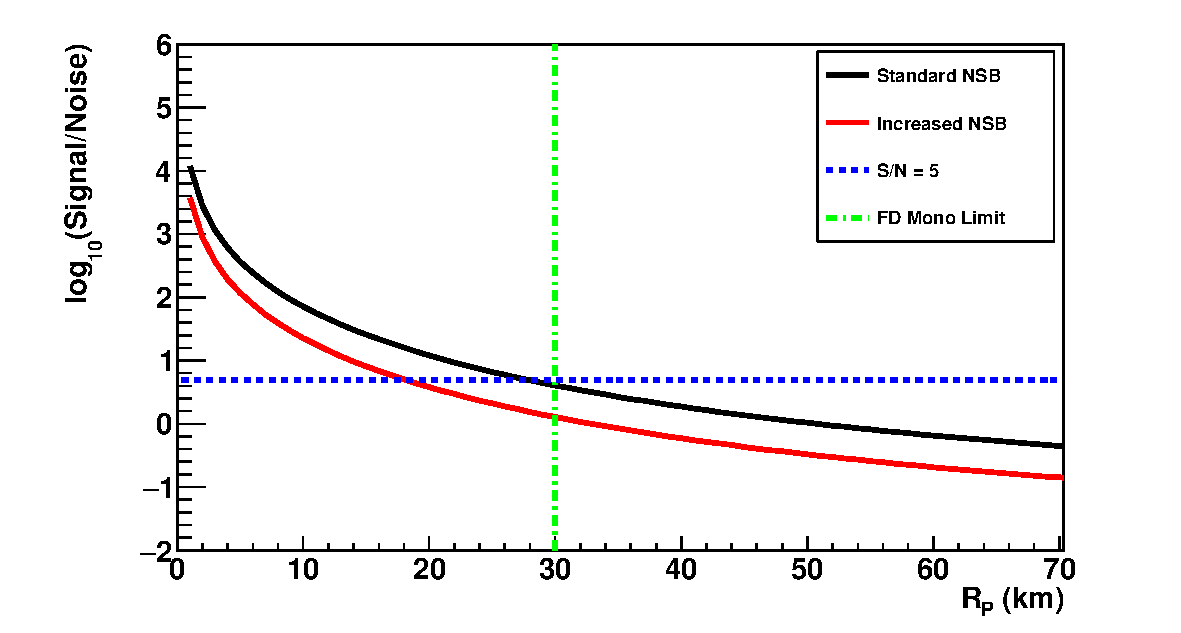
\includegraphics[width=\textwidth]{chapters/graphs/SelectionEff/SignalToNoiseVsDistance_E3e18eV.pdf}
\caption{E = 3 $\times$ 10$^{18}$ eV}
\end{subfigure}
\vspace{3mm}
\begin{subfigure}[b]{0.48\textwidth}
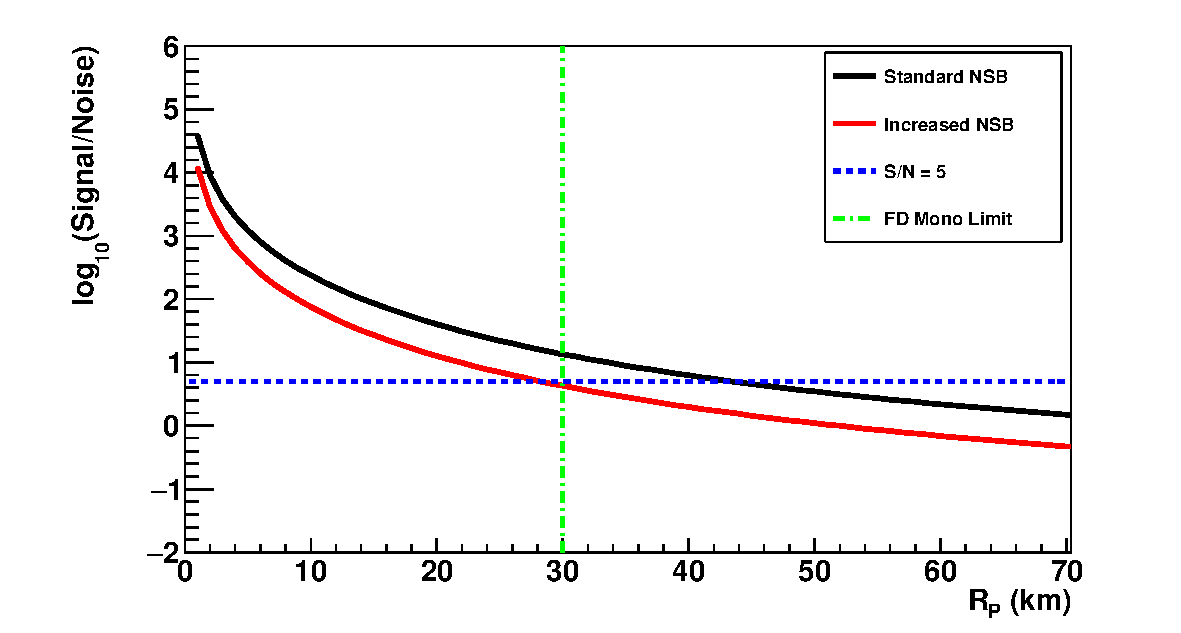
\includegraphics[width=\textwidth]{chapters/graphs/SelectionEff/SignalToNoiseVsDistance_E1e19eV.pdf}
\caption{E = 1 $\times$ 10$^{19}$ eV}
\end{subfigure}
\hspace{3mm}
\begin{subfigure}[b]{0.48\textwidth}
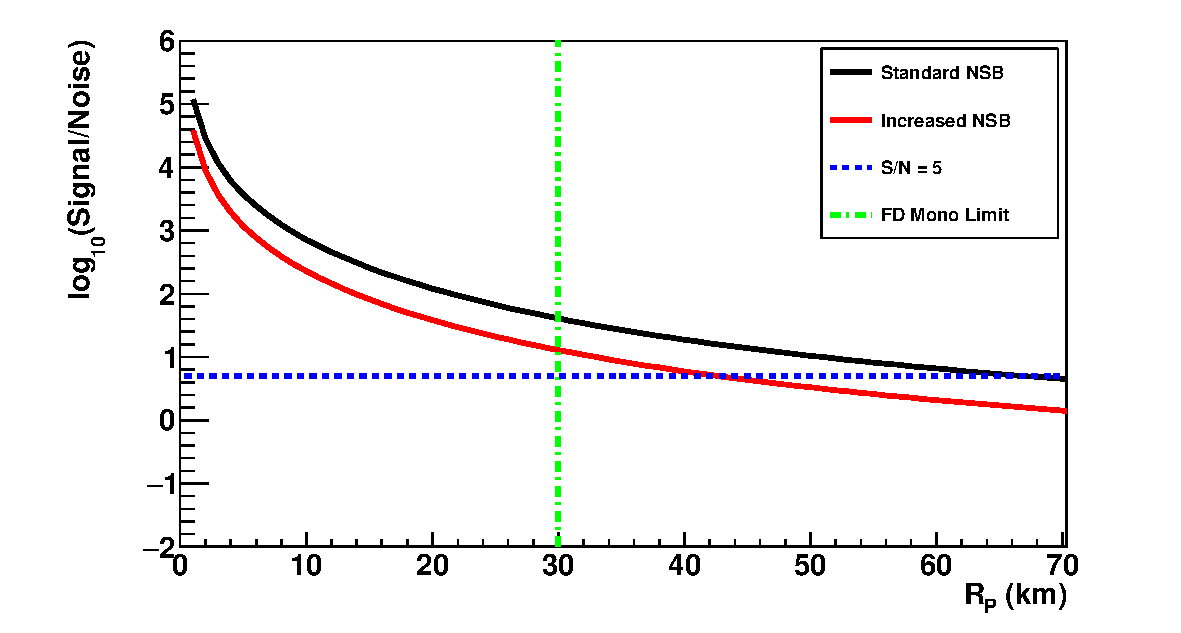
\includegraphics[width=\textwidth]{chapters/graphs/SelectionEff/SignalToNoiseVsDistance_E3e19eV.pdf}
\caption{E = 3 $\times$ 10$^{19}$ eV}
\end{subfigure}
\caption{Using the FD values in Table \ref{tab:FDvalues} and Eq. \ref{eq:SN_complete} to calculate the Signal-to-Noise ratio from specific values for the FD, NSB and conversion's from shower energy to photons to photo-electrons.  The black solid line represents the S/N ratio at typical NSB flux seen at Auger, the red solid line represents the S/N ratio if the NSB flux was increased by a factor of 10, the blue dash line represents the single pixel trigger threshold, and the green dashed line represents the viewing limit of a single FD telescope before an event is closer to another FD telescope. } \label{fig:SNvsDistance}
\end{figure}

The result of calculating the theoretical of the Signal-to-Noise Ratio is shown in Fig. \ref{fig:RangeIncVsRangeStand} and Fig. \ref{fig:RatioAreaVsDistance}. The scale for both is shown in Log$_{10}$ scale so the colour range above and below one is equidistant.  Range$_{\mathrm{Stand}}$ is the expected S/N ratio for the range with standard observed NSB and Range$_{\mathrm{Increase}}$ is the expected S/N for the range with observed NSB increased by a factor of 10. Fig. \ref{fig:RangeIncVsRangeStand} shows the relationship between the S/N ratio for Range$_{\mathrm{Stand}}$ and Range$_{\mathrm{Increase}}$. The solid black line represents the S/N ratio for when the distances are equal. The difference between ratio at the solid black line is 1/$\sqrt{10}$. The dashed black line represents where the S/N ratio are equal. It can be seen that Range$_{\mathrm{Increase}}$ is smaller then Range$_{\mathrm{Stand}}$ which is expected when the NSB has been increased for Range$_{\mathrm{Increase}}$. Fig. \ref{fig:RatioAreaVsDistance} shows how much the observing area changes from Range$_{\mathrm{Stand}}$ to Range$_{\mathrm{Increase}}$. The solid black line denotes where the S/N ratio is the same.

Table \ref{tab:FDvalues} and Eq. \ref{eq:SN_complete} where used to produce Fig. \ref{fig:SNvsDistance} which shows how the S/N ratio changes versus distance for cosmic-rays of four different primary energies. The black solid line represents the S/N ratio at typical NSB flux seen at Auger, the red solid line represents the S/N ratio if the NSB flux was increased by a factor of 10, the blue dash line represents the single pixel trigger threshold, and the green dashed line represents the viewing limit of a single FD telescope before an event is closer to another FD telescope. The figures show that for showers with energies above 3 $\times$ 10$^{19}$ eV that increasing the NSB by a factor of 10 would expect no impact on the FD collecting area. For showers energies of 1 $\times$ 10$^{19}$ eV and below it would be expected that the FD collecting area would be reduced as the NSB is increased.



\section{Increasing NSB in Real Data to evaluate \\ Reconstruction Efficiency}


- Aim

To test the effect of increasing the NSB levels in real data to evaluate the effects on reconstruction efficiency. The reconstruction tool that Auger employs is a internally developed software package called OffLine. OffLine takes selected shower events and goes through the process of finding signals within pixles, and calculating energy and arrival direction. The real data set was the showers used for analysis for ICRC 2015. 

\subsection{Method}

- Take shower set

- add artifical noise to the raw pixel traces

- Use OffLine to reconstruct shower with the increased noise

- Compare Selection Efficiency, Energy resolution and bias, and Xmax resolution and bias.

To evaluate the effects of increased NSB levels on the reconstruction efficiency the data set used for ICRC 2015 had artifical noise add to the raw pixel traces. Once the desired NSB level has been added OffLine is used to reconstruct the shower events again. The results from the standard NSB levels and the increased NSB levels can be compare. I mainly focused on the comparison between Efficiency, Energy resolution and bias, and Xmax resolution and bias. This method allows for any NSB flux levels to be investigated.


The Efficiency is comparison of events that are successfully reconstructed at standard NSB compared to the number of events that are successfully reconstructed at the increasde NSB levels. The Efficiency was calculated with the equation used:
\begin{equation}
\mathrm{Efficiency}_{\mathrm{Data}} = \mathrm{N}^{'}_{\mathrm{SelectData}} \ / \ \mathrm{N}^0_{\mathrm{SelectData}}
\end{equation}
where $\mathrm{N}^{0}_{\mathrm{SelectData}}$ is the number of selected events at the standard NSB level and $\mathrm{N}^{'}_{\mathrm{SelectData}}$ is the number of selected events at the increased NSB
level. 

After the Efficiency was calculated the bias and resolution for Xmax and energy was determined. For real data, the bias is the relative change in the mean of the distributions at increased NSB to the mean of the distributions at standard NSB, both after reconstruction and selection cuts. The bias calculations for real data become:
\begin{eqnarray}
\Delta \mathrm{E}_{\mathrm{Data}} &=& \frac{\mathrm{E}_{\mathrm{IncreasedNSB}} - \mathrm{E}_{\mathrm{StandardNSB}}}{\mathrm{E}_{\mathrm{StandardNSB}}} \label{eq:energybias_data} \\
\Delta \mathrm{Xmax}_{\mathrm{Data}} &=& \mathrm{Xmax}_{\mathrm{IncreasedNSB}} - \mathrm{Xmax}_{\mathrm{StandardNSB}}\label{eq:xmaxbias_data}
\end{eqnarray} 
The energy and Xmax resolution is calculated via:
\begin{eqnarray}
\sigma_{\mathrm{resData}} &=& \left( \frac{1}{\mathrm{N}} \sum \sigma^2_i \right)^{1/2}
\end{eqnarray}
where $\sigma^2_i$ is the reconstructed uncertainty on the individual shower events.

\subsection{Results}

\begin{figure}
\centering
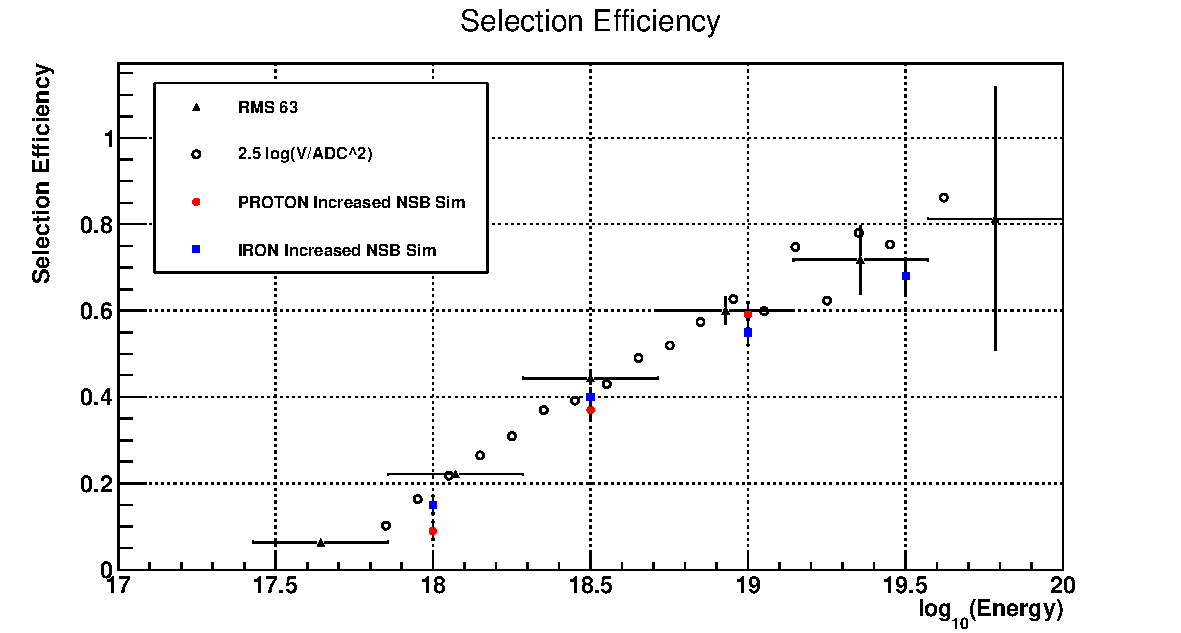
\includegraphics[width=\textwidth]{/home/tsudholz/PhD/Thesis/chapters/graphs/SelectionEff/SelectionEff_errorbars_10timesNSB.pdf}
\caption{The selection efficiency with my repetition against the data points from M. Unger. The method and data sets are similar with the NSB used differing slightly.}
\end{figure}

\begin{figure}
\centering
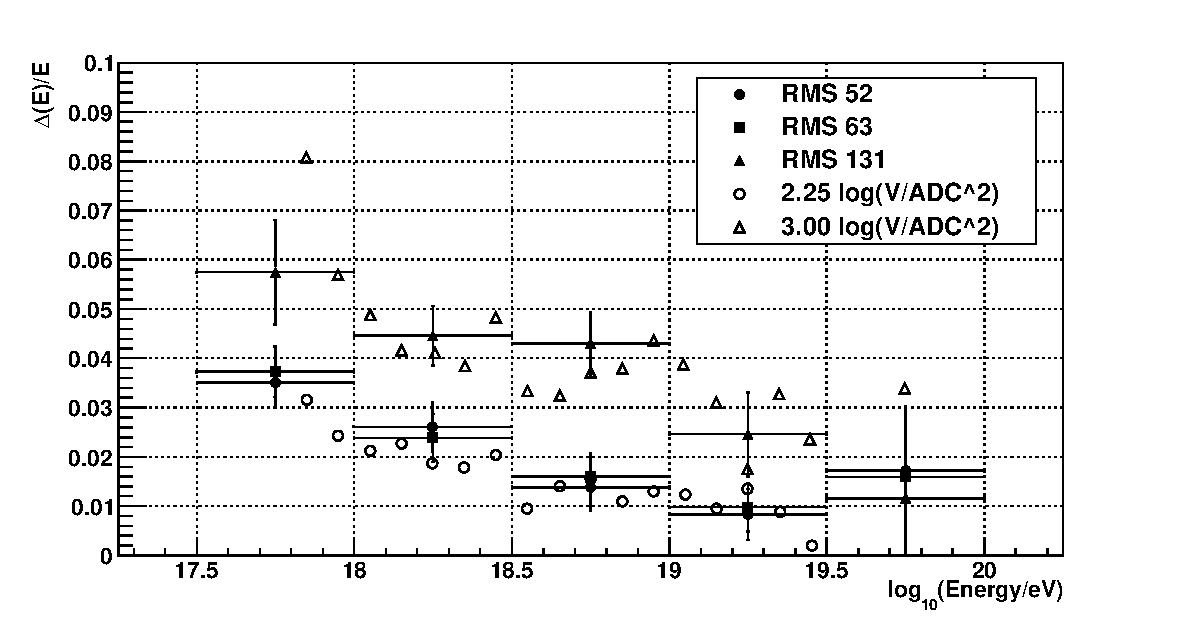
\includegraphics[width=\textwidth]{chapters/graphs/SelectionEff/Smearing_RealData_EnergyBias.pdf}
\caption{Energy Bias from increasing NSB in Real Data.}
\vspace{3mm}
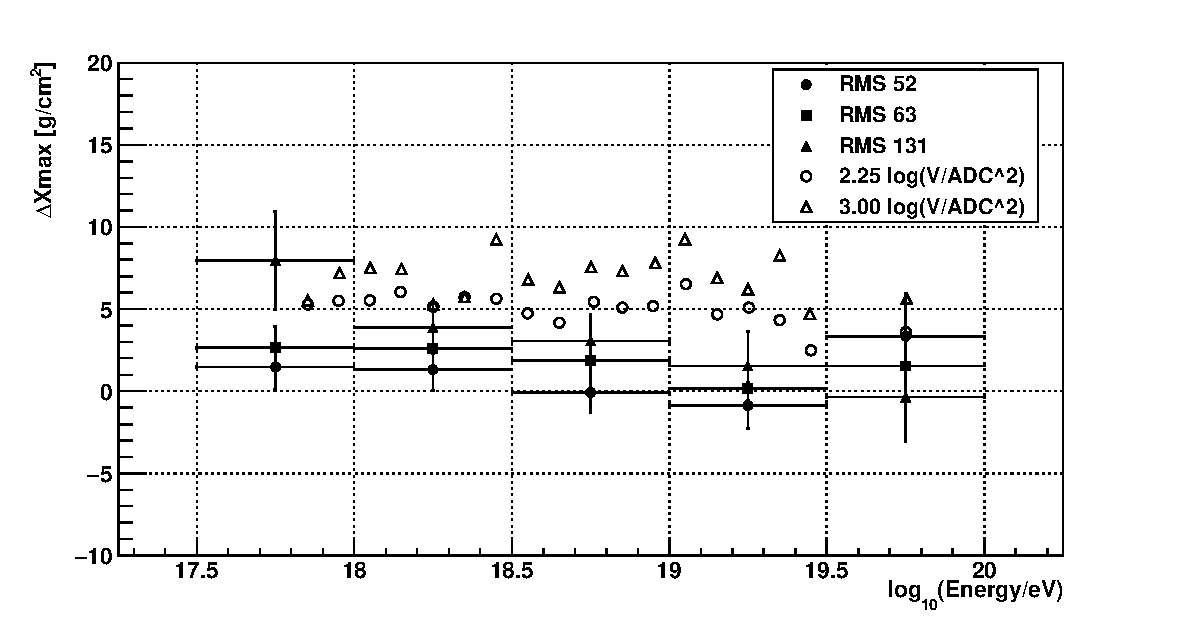
\includegraphics[width=\textwidth]{chapters/graphs/SelectionEff/Smearing_RealData_XmaxBias.pdf}
\caption{Xmax Bias from increasing NSB in Real Data.}
\end{figure}

\begin{figure}
\centering
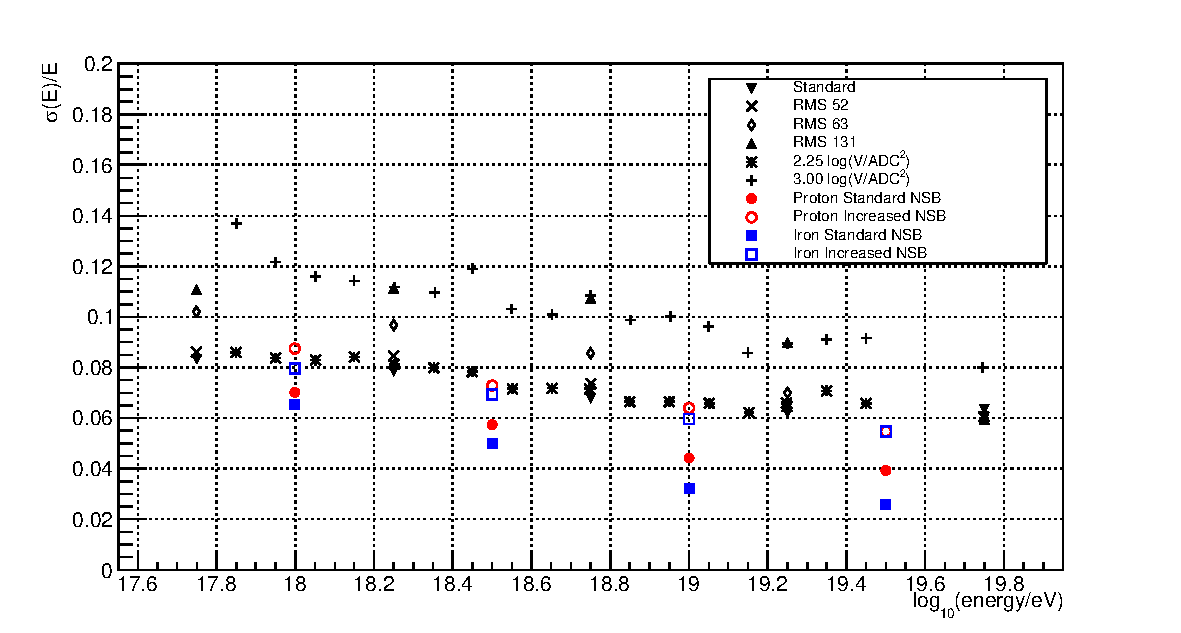
\includegraphics[width=\textwidth]{chapters/graphs/SelectionEff/Combined_EnergyRes_All.pdf}
\caption{Energy Resolution using both Smearing Method data and simulated showers.}
\vspace{3mm}
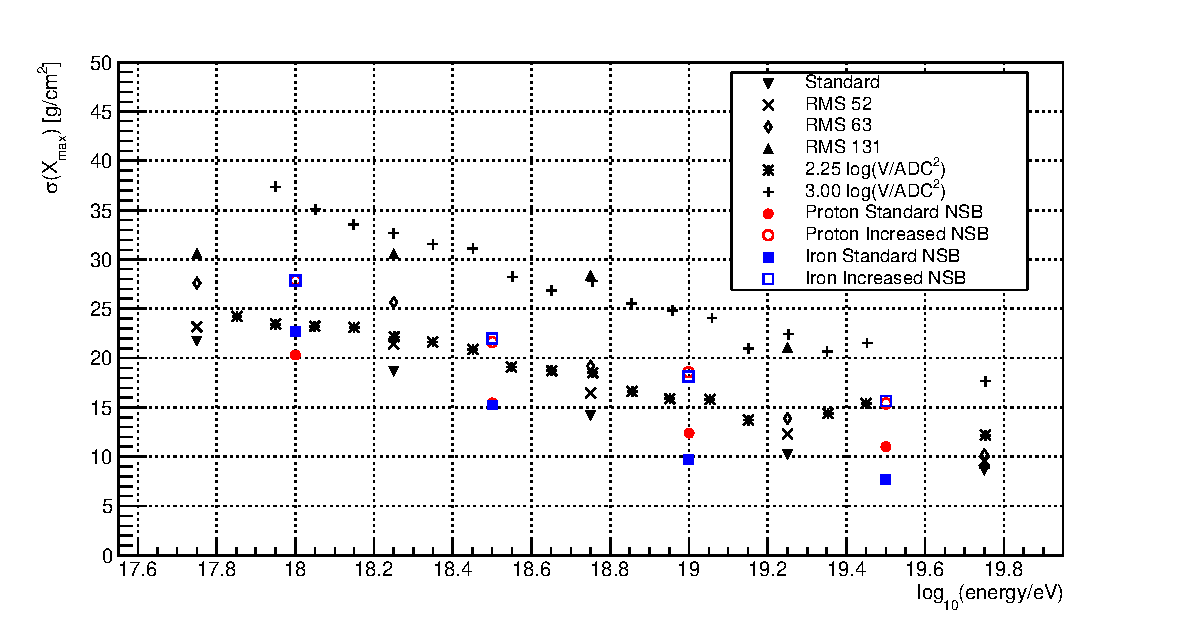
\includegraphics[width=\textwidth]{chapters/graphs/SelectionEff/Combined_XmaxRes_All.pdf}
\caption{Xmax Resolution using both Smearing Method data and simulated showers.}
\end{figure}

\begin{figure}
\centering
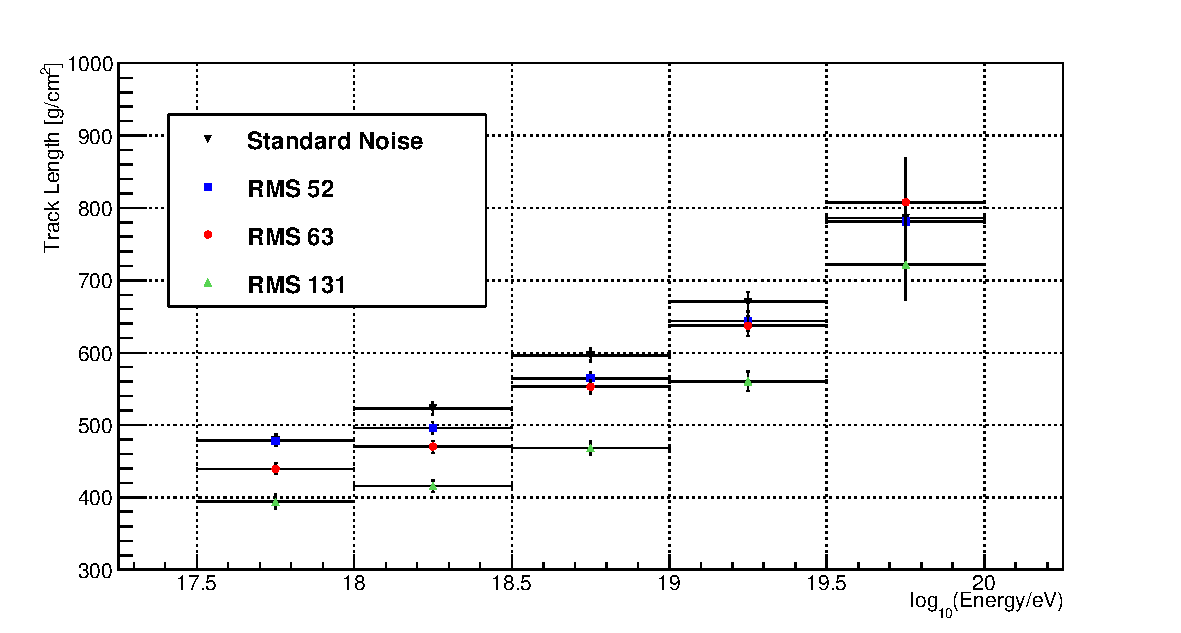
\includegraphics[width=\textwidth]{chapters/graphs/SelectionEff/Smearing_TrackLength_DiffNSBlevels.pdf}
\caption{Track length calculated from events with standard NSB and those with increased NSB fluxes.} \label{fig:TrackLength_Smearing}
\end{figure}

\subsection{Discussion}

\section{Increasing NSB in Simulations to evaluate \\ Trigger/Reconstruction Efficiency}

\subsection{Method}
 The Efficiency was calculated with the equation used:
\begin{equation}
\mathrm{Efficiency} = \mathrm{N}^{'}_{\mathrm{Select}} \ / \ \mathrm{N}^0_{\mathrm{Select}}
\end{equation}
where $\mathrm{N}^{0}_{\mathrm{Select}}$ is the number of selected events at the standard NSB level and $\mathrm{N}^{'}_{\mathrm{Select}}$ is the number of selected events at the increased NSB
level. 

For simulated data the bias is the relative change in the mean of the distributions after the full simulation by EAS events going through an atmosphere with a specified NSB photon field, the FD telescopes optics, trigger, reconstruction and selection cuts compared with Monte-Carlo truth.
\begin{eqnarray}
\Delta \mathrm{E}_{\mathrm{Sim}} &=& \frac{\mathrm{E}_{\mathrm{recon}} - \mathrm{E}_{\mathrm{true}}}{\mathrm{E}_{\mathrm{true}}}  \label{eq:energybias_sim} \\
\Delta \mathrm{Xmax}_{\mathrm{Sim}} &=& \mathrm{Xmax}_{\mathrm{recon}} - \mathrm{Xmax}_{\mathrm{true}} \label{eq:xmaxbias_sim}
\end{eqnarray}
 
 
The energy and Xmax resolution is calculated via:
\begin{eqnarray}
\sigma_{\mathrm{resSim}} &=& \left( \frac{1}{\mathrm{N}} \sum \frac{1}{\sigma^2_i} \right)^{1/2}
\end{eqnarray}

\subsection{Comparison of Simulated Data to Real Data}
\begin{figure}
\centering
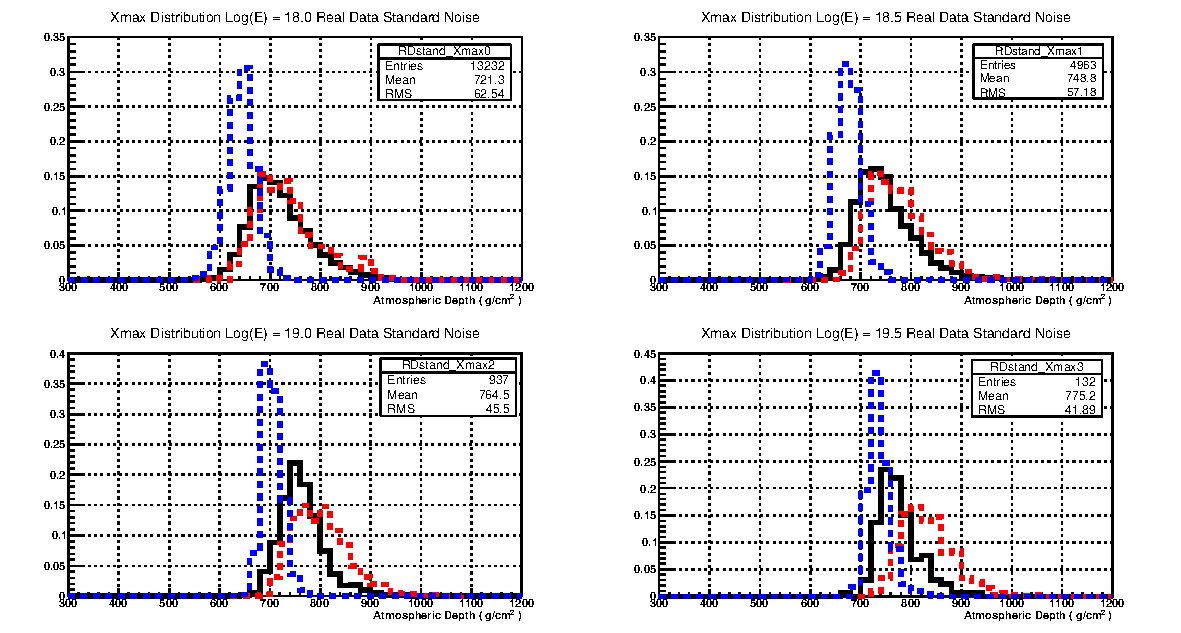
\includegraphics[width=\textwidth]{chapters/graphs/SelectionEff/RealDataAndSim_XmaxDistComp.pdf}
\caption{Distribution of Xmax with Real Data and simulation of proton and iron showers.}
\vspace{3mm}
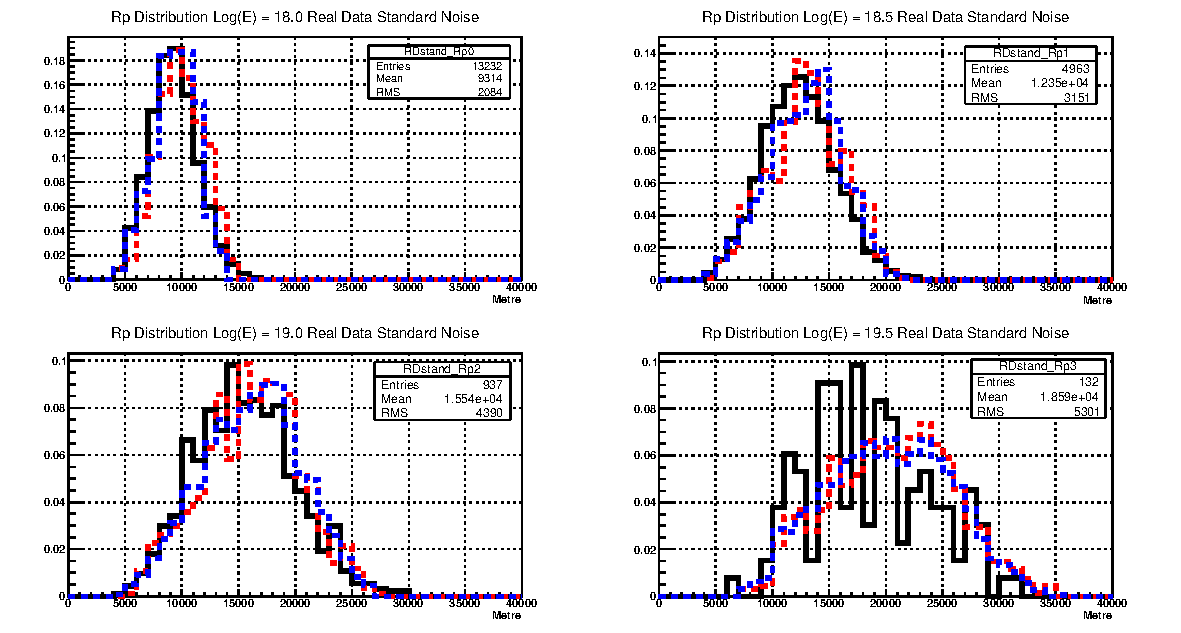
\includegraphics[width=\textwidth]{chapters/graphs/SelectionEff/RealDataAndSim_RpDistComp.pdf}
\caption{Distribution of Rp with Real Data and simulation of proton and iron showers.}
\end{figure}

\begin{figure}
\centering
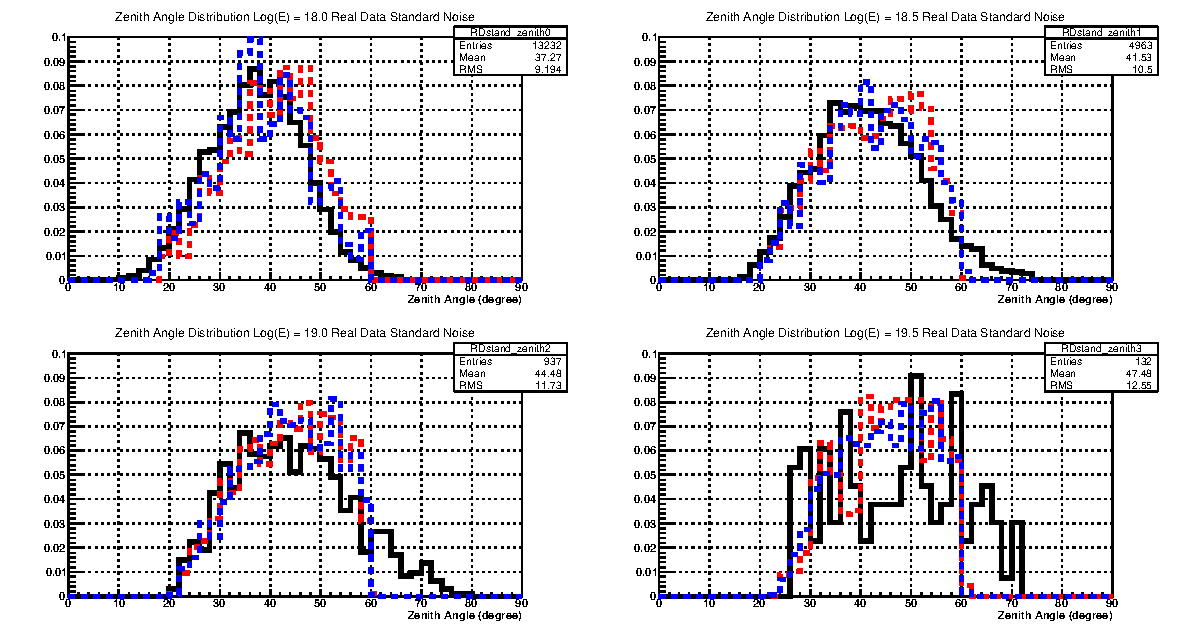
\includegraphics[width=\textwidth]{chapters/graphs/SelectionEff/RealDataAndSim_ZenithDistComp.pdf}
\caption{Distribution of Zenith angle with Real Data and simulation of proton and iron showers.}
\vspace{3mm}
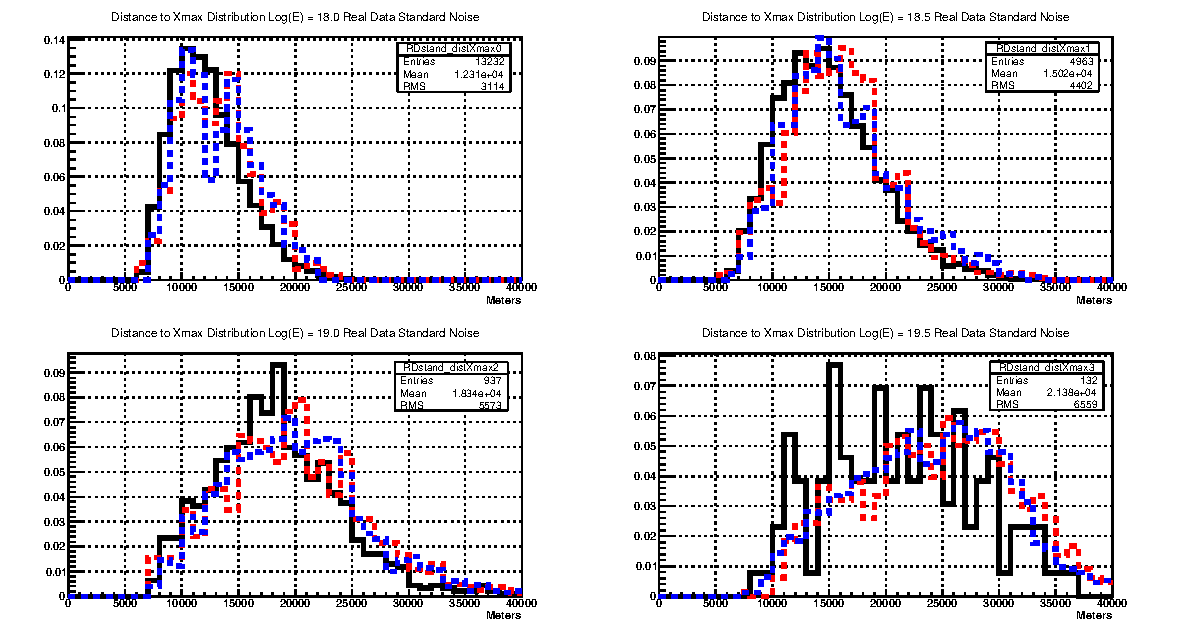
\includegraphics[width=\textwidth]{chapters/graphs/SelectionEff/RealDataAndSim_DistToXmaxDistComp.pdf}
\caption{Distribution of Distance to Xmax with Real Data and simulation of proton and iron showers.}
\end{figure}

\subsection{Results}
\begin{figure}
\centering
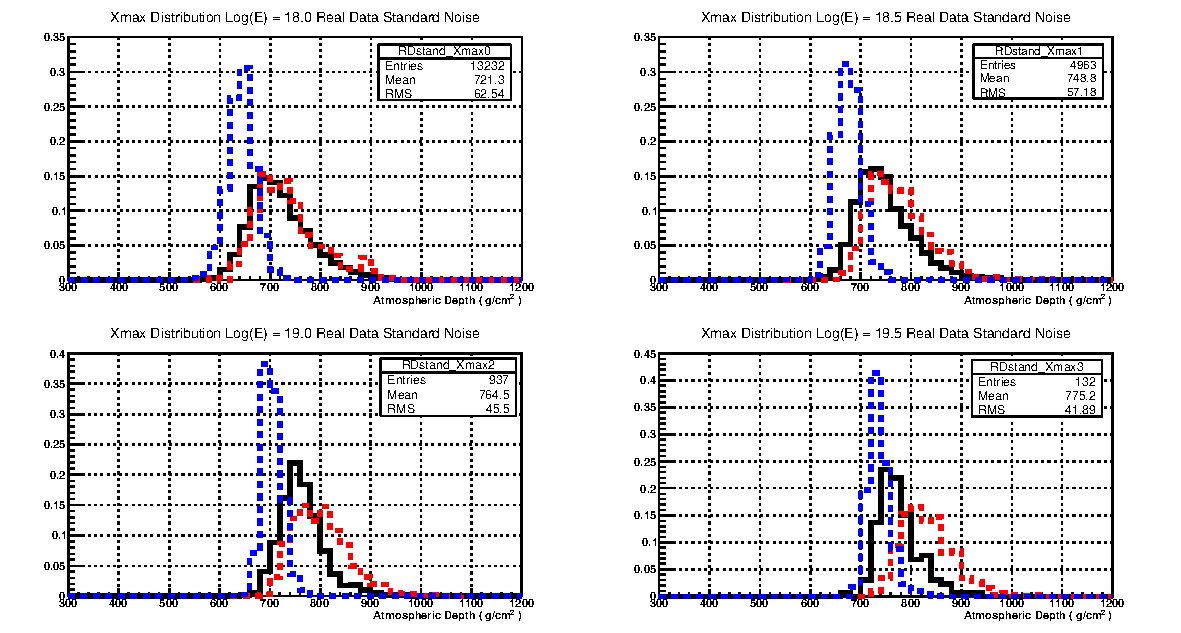
\includegraphics[width=\textwidth]{chapters/graphs/SelectionEff/RealDataAndSim_XmaxDistComp.pdf}
\caption{Distribution of Xmax with Real Data and simulation of proton and iron showers.}
\vspace{3mm}
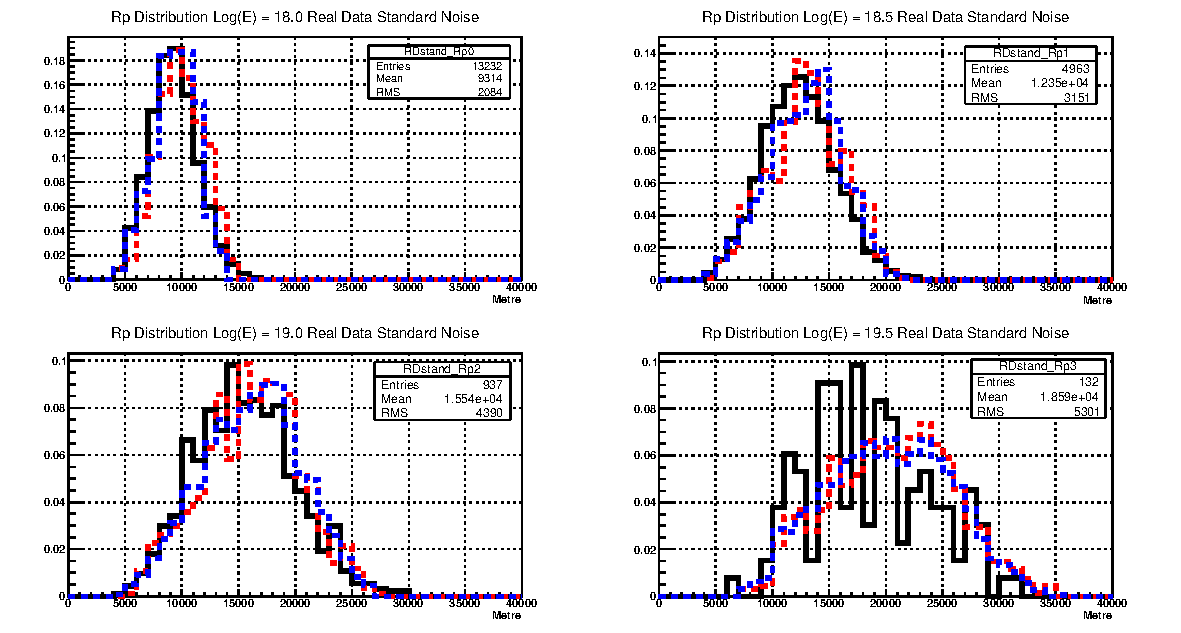
\includegraphics[width=\textwidth]{chapters/graphs/SelectionEff/RealDataAndSim_RpDistComp.pdf}
\caption{Distribution of Rp with Real Data and simulation of proton and iron showers.}
\end{figure}

\begin{figure}
\centering
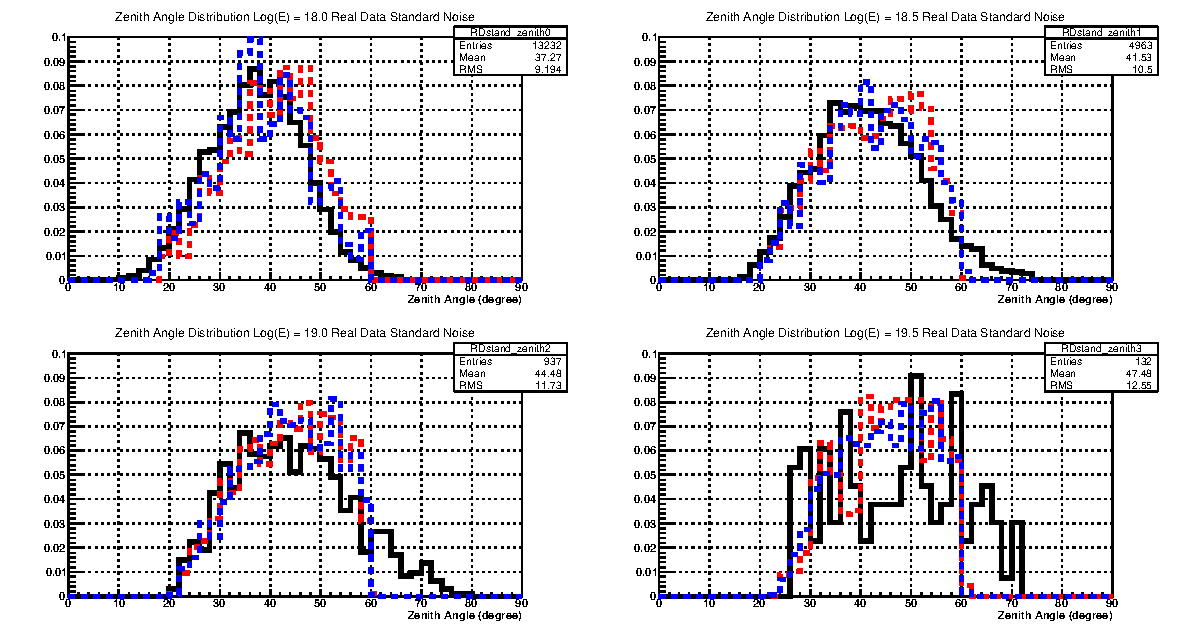
\includegraphics[width=\textwidth]{chapters/graphs/SelectionEff/RealDataAndSim_ZenithDistComp.pdf}
\caption{Distribution of Zenith angle with Real Data and simulation of proton and iron showers.}
\vspace{3mm}
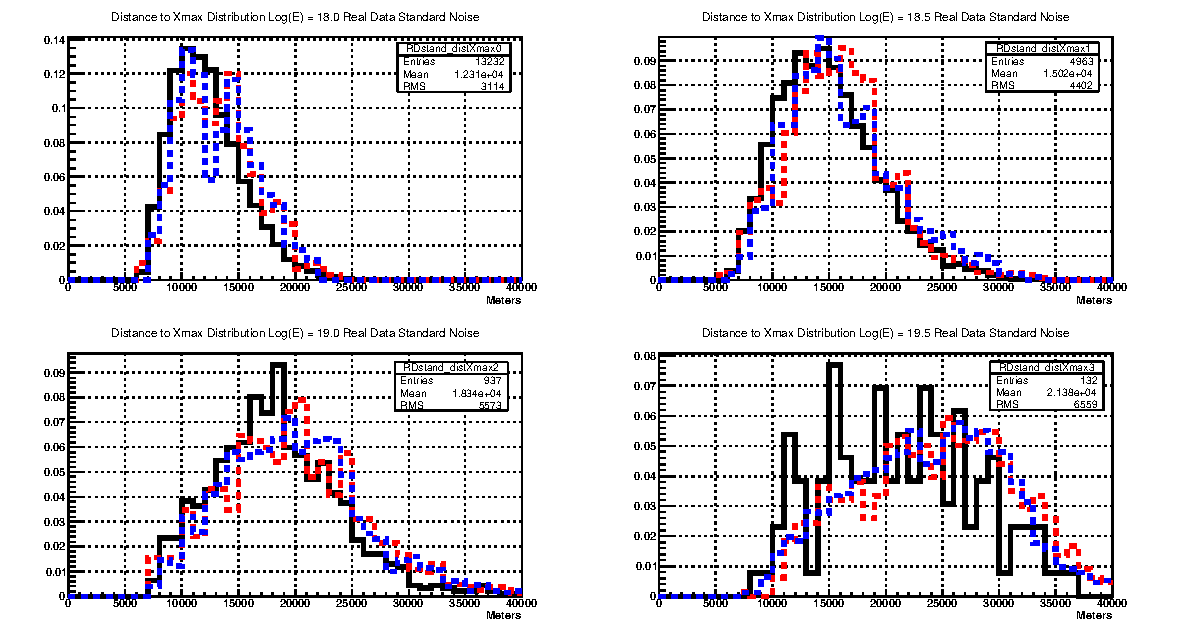
\includegraphics[width=\textwidth]{chapters/graphs/SelectionEff/RealDataAndSim_DistToXmaxDistComp.pdf}
\caption{Distribution of Distance to Xmax with Real Data and simulation of proton and iron showers.}
\end{figure}


\begin{figure}
\centering
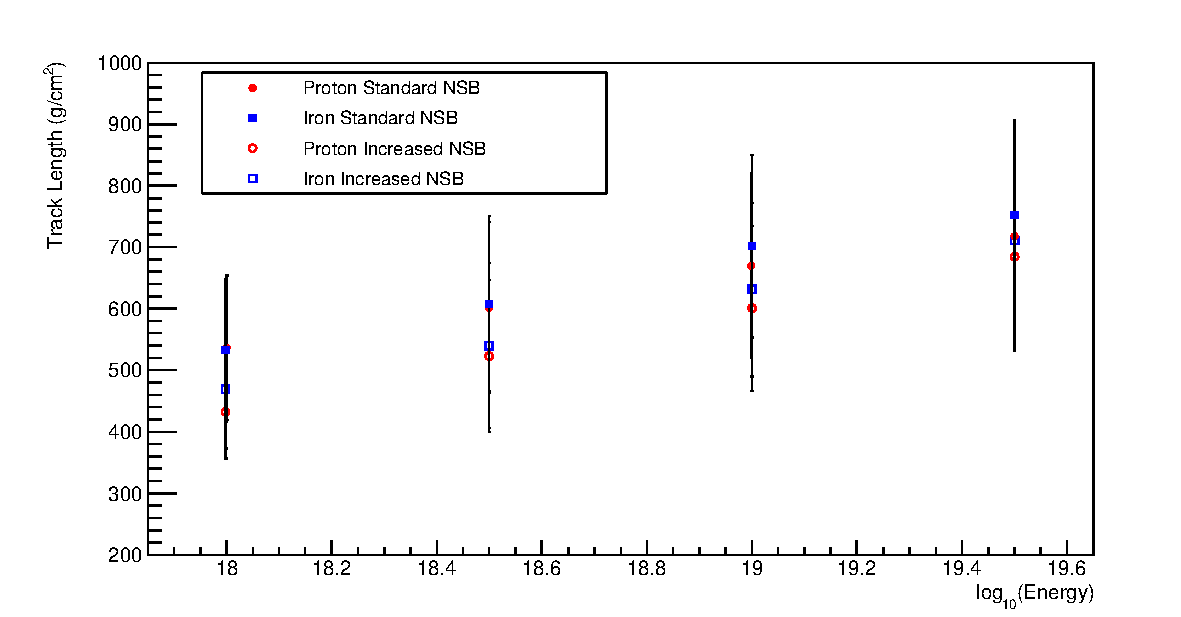
\includegraphics[width=\textwidth]{chapters/graphs/SelectionEff/Simulation_TrackLength_Comb_StandANdIncreasedNSB.pdf}
\caption{Track length using simulation of proton and iron CONEX showers.} \label{fig:TrackLength_Sim}
\end{figure}
\subsection{Discussion}

\section{Conclusion/Summary}
